\documentclass{article}\usepackage[]{graphicx}\usepackage[]{color}
%% maxwidth is the original width if it is less than linewidth
%% otherwise use linewidth (to make sure the graphics do not exceed the margin)
\makeatletter
\def\maxwidth{ %
  \ifdim\Gin@nat@width>\linewidth
    \linewidth
  \else
    \Gin@nat@width
  \fi
}
\makeatother

\definecolor{fgcolor}{rgb}{0.345, 0.345, 0.345}
\newcommand{\hlnum}[1]{\textcolor[rgb]{0.686,0.059,0.569}{#1}}%
\newcommand{\hlstr}[1]{\textcolor[rgb]{0.192,0.494,0.8}{#1}}%
\newcommand{\hlcom}[1]{\textcolor[rgb]{0.678,0.584,0.686}{\textit{#1}}}%
\newcommand{\hlopt}[1]{\textcolor[rgb]{0,0,0}{#1}}%
\newcommand{\hlstd}[1]{\textcolor[rgb]{0.345,0.345,0.345}{#1}}%
\newcommand{\hlkwa}[1]{\textcolor[rgb]{0.161,0.373,0.58}{\textbf{#1}}}%
\newcommand{\hlkwb}[1]{\textcolor[rgb]{0.69,0.353,0.396}{#1}}%
\newcommand{\hlkwc}[1]{\textcolor[rgb]{0.333,0.667,0.333}{#1}}%
\newcommand{\hlkwd}[1]{\textcolor[rgb]{0.737,0.353,0.396}{\textbf{#1}}}%

\usepackage{framed}
\makeatletter
\newenvironment{kframe}{%
 \def\at@end@of@kframe{}%
 \ifinner\ifhmode%
  \def\at@end@of@kframe{\end{minipage}}%
  \begin{minipage}{\columnwidth}%
 \fi\fi%
 \def\FrameCommand##1{\hskip\@totalleftmargin \hskip-\fboxsep
 \colorbox{shadecolor}{##1}\hskip-\fboxsep
     % There is no \\@totalrightmargin, so:
     \hskip-\linewidth \hskip-\@totalleftmargin \hskip\columnwidth}%
 \MakeFramed {\advance\hsize-\width
   \@totalleftmargin\z@ \linewidth\hsize
   \@setminipage}}%
 {\par\unskip\endMakeFramed%
 \at@end@of@kframe}
\makeatother

\definecolor{shadecolor}{rgb}{.97, .97, .97}
\definecolor{messagecolor}{rgb}{0, 0, 0}
\definecolor{warningcolor}{rgb}{1, 0, 1}
\definecolor{errorcolor}{rgb}{1, 0, 0}
\newenvironment{knitrout}{}{} % an empty environment to be redefined in TeX

\usepackage{alltt}
\usepackage{apacite,geometry,fancyhdr}
\pagestyle{fancy}
\rhead{Hurley \& Susmann}
\lhead{\thepage}
\IfFileExists{upquote.sty}{\usepackage{upquote}}{}
\begin{document}





\title{An Analysis of Massachusetts' Standardized Testing through Multi-Group Structural Equation Modelling}
\date{March 24, 2014}
\author{Landon Hurley\\ Psychology, SUNY Geneseo \and Herb Susmann\\ Mathematics, SUNY Geneseo}

\maketitle

\section{Abstract}

\section{Introduction}

\subsection{Data}

The Massachusetts Compreshensive Assessment System (MCAS) is a standardized test administered to Massachusetts public school students in grades 3-10 since 1998. We examine a subset sample of 10\textsuperscript{th} grade students' results from the 2009 Spring MCAS test. The data also contains basic demographic information for each student comprised of race/ethnicity, gender, and an academic engagement questionnaire. Each test consists of multiple choice items and open-ended questions that are graded on a holistic scale, implemented as a 5 point integer scale. 

The examinations are comprised of three separate knowledge domains: English, Mathematics and a science component. Every student takes identical versions of the English and Mathematics sections; the science component can be fulfilled by taking either a Biology, Chemistry, Introductory Physics, or Technology/Engineering test. \cite{mcas_summary}

The MCAS examination structure has received substantial criticism from both educational activists and theoreticians. The former, comprised mainly of teachers and educational policy analysts, claim that the test is unfairly biased against students as a function of demographics, while citing the significant impediment that poor performance upon the tests has upon both immediate and long-term outcomes. Theoretical perspectives on test design are the primary domain of psychometrics, who hold the unfortunate distinction of both supporting standards-based assessment, and subsequently watching their recommendations be ignored when put into practice, either through misinterpretation of statistical results, or the implementation of unrealitic expectations that ignore the original purpose: measurement, or the designation of numerical scales to classify underlying unobservable latent constructs. 

\subsection{Theoretical structure of the test}
Our paper begins with an analaysis of both the psychometric equivalance of the MCAS test within our sample of 10\textsuperscript{th} grade students, followed by an investigration into performance within each knowledge domain, conditioned upon the demographics and item responses found within a questionnaire included with the test.
\section{Methods}
\subsection{Subjects}
Our sample is comprised of 10,515 10\textsuperscript{th} grade students enrolled in Massachusett's public education system, and is assumed to be drawn as an unbiased sample of the total universe of 10\textsuperscript{th} graders. Provided demographics present as follows 4.48\% Asian, 2.97\% Black, 3.63\% Hispanic/Latino, 1.8\% multiracial, 0.17\% Native American, .12\% Pacific Islander, and 86.82\% White; 50.32\% was female, and there are no significant interactions between gender and ethnicity.

Unfortunately for our purposes, the primary point of contention regarding exam disparity, student socio-economic status (SES), was not available, which limits our ability to test and explore the purported causal relaionship with student scores \cite{Gaudet}, as mediated by ethnicity or spatial location. 
\subsection{Procedure}
A critical assumption within standardised testing, and in truth any measurement scale, is that the test demonstrates a psychometric property called measurement invariance/equivalence. This property is a series of mathematical constraints applied to latent variables that are assumed to be non-significantly different between groups. Latent variables are unobservable constructs that underly the observed measures; one typically estiamtes them by computing standard principal axis factor analysis. The constraints serve to empirically demonstrate that across sub-populations, the test measures the same concepts, and that each item tests in a similar way the same construct in comparison to the overall sample, by imposing restrictions in a sequential four phase procedure:
\begin{enumerate}
\item{Configural invariance:} 
Tests whether the same factor model (i.e., latent variables, equivalent to knowledge subdomains, for example grammar) is found within each subgroup.
\item{Weak invariance:}
Tests whether in addition to the same factor structure, the same items load equivalently onto the same same structure.
\item{Strong invariance:}
Tests that the intercepts, item loadings, and factor structure are equivalent across groups.
\item{Strict invariance:}
Tests the assumption that in addition to the preceeding steps, the residual variances are equivalent across groups.
\end{enumerate}
These four factors are argued to be necessary conditions for a fair and equitable comparison\cite{Meredith}, and are established by way of multi-group confirmatory factor analysis (MG-CFA). In this paper, we examine these factors using a group of R packages cited at the end of the paper \cite{psych,lavaan,semTools}. 
Exploratory bootstrapped oblimin factor analyses were conducted upon each section to establish the number of domains and high loading items within each of the three tests. As a consequence of the extreme ethnicity imbalance within three of the four science exams, only Biology was tested using MG-CFA.

Furthermore, we investigated the information found within the questionnaire, relating them to the students' scores on the three sections using both multivariate parametric regressions, and a non-parametric predictive procedure using the mvpart package, which models multivariate regression trees.

Missing data in survey and test data is an important consideration, and there exist a number of techniques to produce more robust solutions, mainly working under the Bayesian estimation process for missing data pioneered by Donald Rubin\cite{rubin}. However, within the structure of the exam, missing data was unsurprisingly a rare occurence: the highest proportion of missing for any item was .008, and 91.23\% had no missing questions. Even so, for the MG-CFA, we attempted to account for this by utilising the Full Information Maximum Likelihood (FIML) estimation, in conjunction with a large number of bootstraps to obtain accurate estimates of asymptotic errors. However, the questionnaire exhibited extreme proportions of non-response, which is problematic for the multivariate regression techniques, producing potentially biased results under the assumption that items are missing completely at random. As such, we processed the original responses using the mice package\cite{mice}, using 25 imputed data frames with 30 iterations in each dataframe. Regression trees are relatively robust to missing data, because all information is not processed simultaneously, but sequentially in order of variable importance, and as such we did not take any additional steps when conducting that analysis.
\section{Results}
\subsection{Exploratory factor analyses}
Given the preceeding information, we examined the Mathematics, English, and Biology sections of the exam, using a oblimin rotated factor structure, with the number of latent factors equal to the number of general domains; factor loadings were calculated using maximum likelihood estimates from the tetrachoric correlation matrices for each subset of items. The psych package was used to calculate the factor structure. Items that loaded higher than .3 on a factor were specified as indicators, and diagrams of each factor can be located in Appendix B.
\subsection{MG-CFA}
As a consequence of the unequal numbers of test takers between Biology and the rest of the science exam options, we chose to run two separate tests for measurement invariance: the first was composed of the total sample on the English and Mathematics, and the second was composed of the Biology testees ($N$=9,239); exploratory factor analyses (EFA) presented the following results:

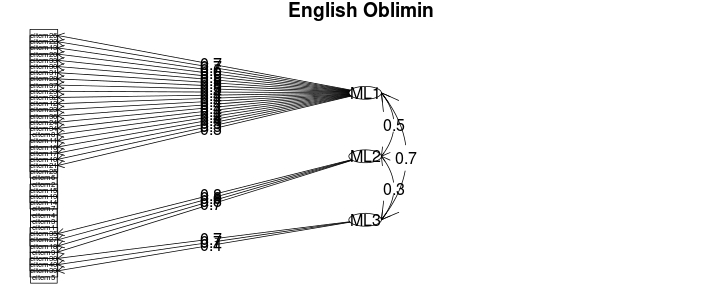
\includegraphics{/home/landon/Documents/workspace/DataCompete/upstat-competition/figure/English.jpeg}

\begin{knitrout}
\definecolor{shadecolor}{rgb}{0.969, 0.969, 0.969}\color{fgcolor}\begin{kframe}
\begin{alltt}
\hlkwd{fa.diagram}\hlstd{(fmat,} \hlkwc{main} \hlstd{=} \hlstr{"Mathematics Oblimin"}\hlstd{)}
\end{alltt}


{\ttfamily\noindent\bfseries\color{errorcolor}{\#\# Error: could not find function "{}fa.diagram"{}}}\end{kframe}
\end{knitrout}


\begin{knitrout}
\definecolor{shadecolor}{rgb}{0.969, 0.969, 0.969}\color{fgcolor}\begin{kframe}
\begin{alltt}
\hlkwd{fa.diagram}\hlstd{(fsci1,} \hlkwc{main} \hlstd{=} \hlstr{"Biology Oblimin"}\hlstd{)}
\end{alltt}


{\ttfamily\noindent\bfseries\color{errorcolor}{\#\# Error: could not find function "{}fa.diagram"{}}}\end{kframe}
\end{knitrout}


These were subsequently specified using a FIML procedure with bootstrapped sampling within the four primary ethnicities: A,B,H,W. Other ethnicities were excluded because of their relative rarity within the sample. As a consequence of the $\chi$\textsuperscript{2} fit statistic, defined as \begin{equation} \chi^2_{d.f}=2(N-1) * F_0 \end{equation} scales as a function of both sample size and the minimum function test statistic $F_0$, traditional measurement invariance, which uses changes in significance to reject a constraint, fails here, as the sample size guarantees significant results. In response to this fact, we employ three different fitness criterion: the $\Delta$ Comparative Fit Index (CFI) \cite{Bentler}, the $\Delta$ root mean square error of approximation (RMSEA), and the $\Delta$ Tucker-Lewis Index (TLI) \cite{Chen}. For all three, decreases in model fit of greater than .01 are considered significant reductions in model fit. In addition, we include An (Akaike) Information Criterion (AIC), to demonstrate whether model fit increases or decreases between sequential steps in comparison to the theoretical true model.

\subsection{English}
The English section constructed using the following system of latent and test items, as predictors of the unstandardized English score, as given below.
\begin{knitrout}
\definecolor{shadecolor}{rgb}{0.969, 0.969, 0.969}\color{fgcolor}\begin{kframe}
\begin{alltt}
\hlstd{e1} \hlkwb{=} \hlopt{~}\hlstd{eitem8} \hlopt{+} \hlstd{eitem10} \hlopt{+} \hlstd{eitem11} \hlopt{+} \hlstd{eitem12} \hlopt{+} \hlstd{eitem13} \hlopt{+} \hlstd{eitem16} \hlopt{+} \hlstd{eitem17} \hlopt{+} \hlstd{eitem20} \hlopt{+}
    \hlstd{eitem21} \hlopt{+} \hlstd{eitem22} \hlopt{+} \hlstd{eitem23} \hlopt{+} \hlstd{eitem24} \hlopt{+} \hlstd{eitem25} \hlopt{+} \hlstd{eitem26} \hlopt{+} \hlstd{eitem28} \hlopt{+} \hlstd{eitem29} \hlopt{+}
    \hlstd{eitem30} \hlopt{+} \hlstd{eitem31} \hlopt{+} \hlstd{eitem32} \hlopt{+} \hlstd{eitem33} \hlopt{+} \hlstd{eitem34} \hlopt{+} \hlstd{eitem36} \hlopt{+} \hlstd{eitem37}
\hlstd{e2} \hlkwb{=} \hlopt{~}\hlstd{eitem27} \hlopt{+} \hlstd{eitem35} \hlopt{+} \hlstd{eitem9} \hlopt{+} \hlstd{eitem18}
\hlstd{e3} \hlkwb{=} \hlopt{~}\hlstd{eitem38} \hlopt{+} \hlstd{eitem39} \hlopt{+} \hlstd{eitem40}
\hlstd{erawsc} \hlopt{~} \hlstd{e1} \hlopt{+} \hlstd{e2} \hlopt{+} \hlstd{e3}
\end{alltt}
\begin{verbatim}
## erawsc ~ e1 + e2 + e3
\end{verbatim}
\end{kframe}
\end{knitrout}


\subsubsection{Configural Invariance}
\begin{knitrout}
\definecolor{shadecolor}{rgb}{0.969, 0.969, 0.969}\color{fgcolor}\begin{kframe}
\begin{alltt}
\hlkwd{fitMeasures}\hlstd{(MI.eng}\hlopt{$}\hlstd{fit.configural,} \hlkwd{c}\hlstd{(}\hlstr{"chisq"}\hlstd{,} \hlstr{"tli"}\hlstd{,} \hlstr{"cfi"}\hlstd{,} \hlstr{"rmsea"}\hlstd{,} \hlstr{"aic"}\hlstd{))}
\end{alltt}


{\ttfamily\noindent\bfseries\color{errorcolor}{\#\# Error: could not find function "{}fitMeasures"{}}}\end{kframe}
\end{knitrout}

As the summary statistics given in the analyses show, configural invariance is supported, meaning that all four ethnicities employ the same conceptual frameworks to answer the test items. 
\subsubsection{Metric (Weak) Invariance}
Weak Invariance does impact the model fit compared to step 1, however negligably: $\Delta$ CFI = .002, $\Delta$ RMSEA =. , $\Delta$$\chi^2$=187.875, and the $\Delta$ TLI =.

\begin{knitrout}
\definecolor{shadecolor}{rgb}{0.969, 0.969, 0.969}\color{fgcolor}\begin{kframe}
\begin{alltt}
\hlkwd{fitMeasures}\hlstd{(MI.eng}\hlopt{$}\hlstd{fit.loadings,} \hlkwd{c}\hlstd{(}\hlstr{"chisq"}\hlstd{,} \hlstr{"tli"}\hlstd{,} \hlstr{"cfi"}\hlstd{,} \hlstr{"rmsea"}\hlstd{,} \hlstr{"aic"}\hlstd{))}
\end{alltt}


{\ttfamily\noindent\bfseries\color{errorcolor}{\#\# Error: could not find function "{}fitMeasures"{}}}\end{kframe}
\end{knitrout}


\subsubsection{Strong Invariance}
Strong Invariance is established using the model fit indexes above and beyond weak invariance: $\Delta$ CFI = .002, $\Delta$ RMSEA = .000 , and the $\Delta$ TLI =.000 and $\Delta$$\chi^2$=187.875.
\begin{knitrout}
\definecolor{shadecolor}{rgb}{0.969, 0.969, 0.969}\color{fgcolor}\begin{kframe}
\begin{alltt}
\hlkwd{fitMeasures}\hlstd{(MI.eng}\hlopt{$}\hlstd{fit.intercepts,} \hlkwd{c}\hlstd{(}\hlstr{"chisq"}\hlstd{,} \hlstr{"tli"}\hlstd{,} \hlstr{"cfi"}\hlstd{,} \hlstr{"rmsea"}\hlstd{,} \hlstr{"aic"}\hlstd{))}
\end{alltt}


{\ttfamily\noindent\bfseries\color{errorcolor}{\#\# Error: could not find function "{}fitMeasures"{}}}\end{kframe}
\end{knitrout}


\subsubsection{Strict Invariance}
Strict invariance does not hold, with a significant $\Delta$ CFI = .034, $\Delta$ RMSEA = .006, $\Delta$$\chi^2$=1670.297, and the $\Delta$ TLI = .03 indicating lack of fit.
\begin{knitrout}
\definecolor{shadecolor}{rgb}{0.969, 0.969, 0.969}\color{fgcolor}\begin{kframe}
\begin{alltt}
\hlkwd{fitMeasures}\hlstd{(MI.eng}\hlopt{$}\hlstd{fit.residuals,} \hlkwd{c}\hlstd{(}\hlstr{"chisq"}\hlstd{,} \hlstr{"tli"}\hlstd{,} \hlstr{"cfi"}\hlstd{,} \hlstr{"rmsea"}\hlstd{,} \hlstr{"aic"}\hlstd{))}
\end{alltt}


{\ttfamily\noindent\bfseries\color{errorcolor}{\#\# Error: could not find function "{}fitMeasures"{}}}\end{kframe}
\end{knitrout}

\subsection{Mathematics}
While the EFA presented a good model fit for a five factor model, when the SEM model imposed upon the data, it failed to converge due to underspecification. As such, factor 5 was removed, because it consisted of only four low loading items.
\begin{knitrout}
\definecolor{shadecolor}{rgb}{0.969, 0.969, 0.969}\color{fgcolor}\begin{kframe}
\begin{alltt}
\hlstd{m1} \hlkwb{=} \hlopt{~}\hlstd{mitem4} \hlopt{+} \hlstd{mitem5} \hlopt{+} \hlstd{mitem8} \hlopt{+} \hlstd{mitem11} \hlopt{+} \hlstd{mitem12} \hlopt{+} \hlstd{mitem14} \hlopt{+} \hlstd{mitem25} \hlopt{+} \hlstd{mitem32} \hlopt{+}
    \hlstd{mitem35} \hlopt{+} \hlstd{mitem37} \hlopt{+} \hlstd{mitem40} \hlopt{+} \hlstd{mitem42}
\hlstd{m2} \hlkwb{=} \hlopt{~}\hlstd{mitem6} \hlopt{+} \hlstd{mitem10} \hlopt{+} \hlstd{mitem17} \hlopt{+} \hlstd{mitem24} \hlopt{+} \hlstd{mitem39}
\hlstd{m3} \hlkwb{=} \hlopt{~}\hlstd{mitem22} \hlopt{+} \hlstd{mitem28} \hlopt{+} \hlstd{mitem34} \hlopt{+} \hlstd{mitem38} \hlopt{+} \hlstd{mitem41}
\hlstd{m4} \hlkwb{=} \hlopt{~}\hlstd{mitem18} \hlopt{+} \hlstd{mitem20} \hlopt{+} \hlstd{mitem21} \hlopt{+} \hlstd{mitem31} \hlopt{+} \hlstd{mitem42}
\hlstd{mrawsc} \hlopt{~} \hlstd{m1} \hlopt{+} \hlstd{m2} \hlopt{+} \hlstd{m3} \hlopt{+} \hlstd{m4}
\end{alltt}
\begin{verbatim}
## mrawsc ~ m1 + m2 + m3 + m4
\end{verbatim}
\end{kframe}
\end{knitrout}


\subsubsection{Configural Invariance}
\begin{knitrout}
\definecolor{shadecolor}{rgb}{0.969, 0.969, 0.969}\color{fgcolor}\begin{kframe}
\begin{alltt}
\hlkwd{fitMeasures}\hlstd{(MI.maths}\hlopt{$}\hlstd{fit.configural,} \hlkwd{c}\hlstd{(}\hlstr{"chisq"}\hlstd{,} \hlstr{"tli"}\hlstd{,} \hlstr{"cfi"}\hlstd{,} \hlstr{"rmsea"}\hlstd{,} \hlstr{"aic"}\hlstd{))}
\end{alltt}


{\ttfamily\noindent\bfseries\color{errorcolor}{\#\# Error: could not find function "{}fitMeasures"{}}}\end{kframe}
\end{knitrout}

As the summary statistics given in the analyses show, configural invariance is supported, meaning that all four ethnicities employ the same conceptual frameworks to answer the test items. 
\subsubsection{Metric (Weak) Invariance}
Weak Invariance does impact the model fit compared to step 1, however negligably: $\Delta$ CFI = .004, $\Delta$ RMSEA = .001 , $\Delta$$\chi^2$=260.076, and the $\Delta$ TLI = .002.

\begin{knitrout}
\definecolor{shadecolor}{rgb}{0.969, 0.969, 0.969}\color{fgcolor}\begin{kframe}
\begin{alltt}
\hlkwd{fitMeasures}\hlstd{(MI.maths}\hlopt{$}\hlstd{fit.loadings,} \hlkwd{c}\hlstd{(}\hlstr{"chisq"}\hlstd{,} \hlstr{"tli"}\hlstd{,} \hlstr{"cfi"}\hlstd{,} \hlstr{"rmsea"}\hlstd{,} \hlstr{"aic"}\hlstd{))}
\end{alltt}


{\ttfamily\noindent\bfseries\color{errorcolor}{\#\# Error: could not find function "{}fitMeasures"{}}}\end{kframe}
\end{knitrout}


\subsubsection{Strong Invariance}
Strong Invariance does not substantively change model fit above and beyond weak invariance: $\Delta$ CFI = .002, $\Delta$ RMSEA = .000, the $\Delta$ TLI = .000 and $\Delta$$\chi^2$=167.652. 

\begin{knitrout}
\definecolor{shadecolor}{rgb}{0.969, 0.969, 0.969}\color{fgcolor}\begin{kframe}
\begin{alltt}
\hlkwd{fitMeasures}\hlstd{(MI.maths}\hlopt{$}\hlstd{fit.intercepts,} \hlkwd{c}\hlstd{(}\hlstr{"chisq"}\hlstd{,} \hlstr{"tli"}\hlstd{,} \hlstr{"cfi"}\hlstd{,} \hlstr{"rmsea"}\hlstd{,} \hlstr{"aic"}\hlstd{))}
\end{alltt}


{\ttfamily\noindent\bfseries\color{errorcolor}{\#\# Error: could not find function "{}fitMeasures"{}}}\end{kframe}
\end{knitrout}


\subsubsection{Strict Invariance}
Strong Invariance imposes a significant constraint upon model fit: $\Delta$ CFI = .017, $\Delta$ RMSEA = .005, the $\Delta$ TLI = .014 and $\Delta$$\chi^2$=998.348. 

\begin{knitrout}
\definecolor{shadecolor}{rgb}{0.969, 0.969, 0.969}\color{fgcolor}\begin{kframe}
\begin{alltt}
\hlkwd{fitMeasures}\hlstd{(MI.maths}\hlopt{$}\hlstd{fit.residuals,} \hlkwd{c}\hlstd{(}\hlstr{"chisq"}\hlstd{,} \hlstr{"tli"}\hlstd{,} \hlstr{"cfi"}\hlstd{,} \hlstr{"rmsea"}\hlstd{,} \hlstr{"aic"}\hlstd{))}
\end{alltt}


{\ttfamily\noindent\bfseries\color{errorcolor}{\#\# Error: could not find function "{}fitMeasures"{}}}\end{kframe}
\end{knitrout}


\subsection{Biology}
We proceeded with the same methodology to test the science section in isolation, using identical $\Delta$ constraints as above. The test for configural invariance produced non-significant results, indicating general acceptance of the factor structure. In addition, each subsequent test produced similar results, indicating that across all four primary ethnicities, the test operated with equivalent measurement. Biology as presented an interpretable factor structure, which was represented with the following mathematical structure.
\begin{knitrout}
\definecolor{shadecolor}{rgb}{0.969, 0.969, 0.969}\color{fgcolor}\begin{kframe}
\begin{alltt}
\hlstd{s1} \hlkwb{=} \hlopt{~}\hlstd{sitem1} \hlopt{+} \hlstd{sitem2} \hlopt{+} \hlstd{sitem13} \hlopt{+} \hlstd{sitem14} \hlopt{+} \hlstd{sitem15} \hlopt{+} \hlstd{sitem22} \hlopt{+} \hlstd{sitem27} \hlopt{+} \hlstd{sitem30} \hlopt{+}
    \hlstd{sitem33} \hlopt{+} \hlstd{sitem34} \hlopt{+} \hlstd{sitem37} \hlopt{+} \hlstd{sitem40} \hlopt{+} \hlstd{sitem41}
\hlstd{s2} \hlkwb{=} \hlopt{~}\hlstd{sitem3} \hlopt{+} \hlstd{sitem5} \hlopt{+} \hlstd{sitem18} \hlopt{+} \hlstd{sitem19} \hlopt{+} \hlstd{sitem28} \hlopt{+} \hlstd{sitem31} \hlopt{+} \hlstd{sitem35} \hlopt{+} \hlstd{sitem43} \hlopt{+}
    \hlstd{sitem45}
\hlstd{s3} \hlkwb{=} \hlopt{~}\hlstd{sitem8} \hlopt{+} \hlstd{sitem10} \hlopt{+} \hlstd{sitem11} \hlopt{+} \hlstd{sitem12} \hlopt{+} \hlstd{sitem23} \hlopt{+} \hlstd{sitem24} \hlopt{+} \hlstd{sitem25} \hlopt{+} \hlstd{sitem23}
\hlstd{s4} \hlkwb{=} \hlopt{~}\hlstd{sitem4} \hlopt{+} \hlstd{sitem23} \hlopt{+} \hlstd{sitem29} \hlopt{+} \hlstd{sitem32} \hlopt{+} \hlstd{sitem44}
\hlstd{srawsc} \hlopt{~} \hlstd{s1} \hlopt{+} \hlstd{s2} \hlopt{+} \hlstd{s3} \hlopt{+} \hlstd{s4}
\end{alltt}
\begin{verbatim}
## srawsc ~ s1 + s2 + s3 + s4
\end{verbatim}
\end{kframe}
\end{knitrout}


\subsubsection{Configural Invariance}
\begin{knitrout}
\definecolor{shadecolor}{rgb}{0.969, 0.969, 0.969}\color{fgcolor}\begin{kframe}
\begin{alltt}
\hlkwd{fitMeasures}\hlstd{(MI.eng}\hlopt{$}\hlstd{fit.configural,} \hlkwd{c}\hlstd{(}\hlstr{"chisq"}\hlstd{,} \hlstr{"tli"}\hlstd{,} \hlstr{"cfi"}\hlstd{,} \hlstr{"rmsea"}\hlstd{,} \hlstr{"aic"}\hlstd{))}
\end{alltt}


{\ttfamily\noindent\bfseries\color{errorcolor}{\#\# Error: could not find function "{}fitMeasures"{}}}\end{kframe}
\end{knitrout}

As the summary statistics given in the analyses show, configural invariance is supported, meaning that all four ethnicities employ the same conceptual frameworks to answer the test items. 
\subsubsection{Metric (Weak) Invariance}
Weak Invariance does impact the model fit compared to step 1, however negligably: $\Delta$ CFI = .002, $\Delta$ RMSEA = .000 , $\Delta$$\chi^2$=168.330, and the $\Delta$ TLI = .000.

\begin{knitrout}
\definecolor{shadecolor}{rgb}{0.969, 0.969, 0.969}\color{fgcolor}\begin{kframe}
\begin{alltt}
\hlkwd{fitMeasures}\hlstd{(MI.eng}\hlopt{$}\hlstd{fit.loadings,} \hlkwd{c}\hlstd{(}\hlstr{"chisq"}\hlstd{,} \hlstr{"tli"}\hlstd{,} \hlstr{"cfi"}\hlstd{,} \hlstr{"rmsea"}\hlstd{,} \hlstr{"aic"}\hlstd{))}
\end{alltt}


{\ttfamily\noindent\bfseries\color{errorcolor}{\#\# Error: could not find function "{}fitMeasures"{}}}\end{kframe}
\end{knitrout}


\subsubsection{Strong Invariance}
Strong Invariance does fails to substantively change model fit above and beyond metric invariance: $\Delta$ CFI = .002, $\Delta$ RMSEA = .000 , and the $\Delta$ TLI = .000 and $\Delta$$\chi^2$=187.875. 
\begin{knitrout}
\definecolor{shadecolor}{rgb}{0.969, 0.969, 0.969}\color{fgcolor}\begin{kframe}
\begin{alltt}
\hlkwd{fitMeasures}\hlstd{(MI.eng}\hlopt{$}\hlstd{fit.intercepts,} \hlkwd{c}\hlstd{(}\hlstr{"chisq"}\hlstd{,} \hlstr{"tli"}\hlstd{,} \hlstr{"cfi"}\hlstd{,} \hlstr{"rmsea"}\hlstd{,} \hlstr{"aic"}\hlstd{))}
\end{alltt}


{\ttfamily\noindent\bfseries\color{errorcolor}{\#\# Error: could not find function "{}fitMeasures"{}}}\end{kframe}
\end{knitrout}


\subsubsection{Strict Invariance}
Strict Invariance does substantively change model fit above and beyond strong invariance: $\Delta$ CFI = .034, $\Delta$ RMSEA = .006 , and the $\Delta$ TLI = .03 and $\Delta$$\chi^2$=1670.297. 
\begin{knitrout}
\definecolor{shadecolor}{rgb}{0.969, 0.969, 0.969}\color{fgcolor}\begin{kframe}
\begin{alltt}
\hlkwd{fitMeasures}\hlstd{(MI.eng}\hlopt{$}\hlstd{fit.residuals,} \hlkwd{c}\hlstd{(}\hlstr{"chisq"}\hlstd{,} \hlstr{"tli"}\hlstd{,} \hlstr{"cfi"}\hlstd{,} \hlstr{"rmsea"}\hlstd{,} \hlstr{"aic"}\hlstd{))}
\end{alltt}


{\ttfamily\noindent\bfseries\color{errorcolor}{\#\# Error: could not find function "{}fitMeasures"{}}}\end{kframe}
\end{knitrout}


\subsection{Questionnaire}
\subsubsection{Multivariate Regression Tree}

Without preexisting beliefs about the nature of the relationship between the response surface and the questionnaire and demographics, we chose to begin the analyses with an undirected multivariate tree regression \cite{De'ath}, conceptually similar to running a multinomial regression upon the different clusters analysis groups of the response variables. The tree also tests by default the possibility that which science test a student takes interacts with other outcomes --in addition, forcibly partitioning the data does not meaningfully increase model fit. We also made the decision to leave non-response as a legitimate factor level: this allows us to incorporate nonresponse as a partitioning criterion.

\begin{knitrout}
\definecolor{shadecolor}{rgb}{0.969, 0.969, 0.969}\color{fgcolor}\begin{kframe}
\begin{alltt}
\hlkwd{require}\hlstd{(mvpart)}
\end{alltt}


{\ttfamily\noindent\itshape\color{messagecolor}{\#\# Loading required package: mvpart}}\begin{alltt}
\hlkwd{mvpart}\hlstd{(}\hlkwd{cbind}\hlstd{(mrawsc, erawsc, srawsc)} \hlopt{~} \hlstd{.,} \hlkwc{data} \hlstd{= d4)}
\end{alltt}


{\ttfamily\noindent\bfseries\color{errorcolor}{\#\# Error: object 'd4' not found}}\end{kframe}
\end{knitrout}


These results indicate substantive effects between the future student aspirations (those who intended to attain a baccalaureate degree) and overall performance, with these students performing significantly better on all three sections. The failure for the function to further discretize the low achievers indicates that the individual differences wihin accounted for no additional information. For high aspiring students, ethnicity was found to be the second most important in discriminating test scores, with Blacks, Hispanics and Native Americans performing similarly worse on the Mathematics and Biology sections than the other ethnicities. The final node split discriminates between high and low scoring science students, with those who responded as rarely using scientific instruments performing worse. Cross-validated errors were high, at CVE=.905, which corresponds to $R^2$=.15
\subsubsection{Multivariate Regression}
A parametric regression model was also conducted exploring only main effects between the predictors and response.


\section{Discussion}
As indicated in the results section, the test fails to perform equivalently across the four groups, which is the primary point of order in test design and advocacy. Moreover, strict invariance has a specific import upon the function of psychometric and education measurements, testing whether the error variances --the portions of item variation not attributable to the common factors. Conceptually, strict invariance validates the assumption that error variances are different across groups; if this fails, there are either different variables operating on the measures across groups or the same set of variables operates differently across groups \cite{deshon}. This fundamentally demonstrates the importance of ensuring that all four mainstays of measurement invariance be substantiated, especially when one considers the long standing view that residuals convey meaning of unmeasured latent constructs' effects, moderated by group membership in this case \cite{cronbach}. This lends substantive credence to the argument that there are fundamental flaws within the test, specifically with reflection towards students' socioeconomic status.



\bibliography{references}{}
\bibliographystyle{apacite}


\end{document}
